% JSS Article Template
\documentclass{article}


%%% Additional Packages %%%

% Algorithms
% http://tex.stackexchange.com/questions/229355/algorithm-algorithmic-algorithmicx-algorithm2e-algpseudocode-confused
\usepackage{algorithm}% http://ctan.org/pkg/algorithms
\usepackage{algpseudocode}% http://ctan.org/pkg/algorithmicx


% Font stuff
\usepackage[T1]{fontenc}% for correct hyphenation and T1 encoding
%\usepackage{lmodern}% latin modern font
\usepackage[american]{babel}% for American English

% Math fonts/symbols
\usepackage{amsmath}% sophisticated mathematical formulas with amstex (includes \text{})
\usepackage{mathtools}% fix amsmath deficiencies
\usepackage{amssymb}% sophisticated mathematical symbols with amstex
\usepackage{amstext}% ams mathematical fonts
\usepackage{amsfonts}% ams mathematical fonts

% Figures
\usepackage{graphicx}% for including figures

%%% Commands %%%%%%%%%%%%%%%%%%%%%%%%%%%%%%%%%%%%%%%%%%%%%%%%%%%%%%%%%%%%%%%%%%%

% vetors
\newcommand{\ve}[1]{\mathbf{#1}}           % for vetors
\newcommand{\sv}[1]{\boldsymbol{#1}}   % for greek letters
\newcommand{\m}[1]{\mathbf{#1}}               % for matrices
\newcommand{\sm}[1]{\boldsymbol{#1}}   % for greek letters
\newcommand{\tr}[1]{{#1}^{\mkern-1.5mu\mathsf{T}}}              % for transpose
\newcommand{\norm}[1]{||{#1}||}              % for transpose
\newcommand*{\mve}{\operatorname{ve}}
\newcommand*{\trace}{\operatorname{trace}}
\newcommand*{\rank}{\operatorname{rank}}
\newcommand*{\diag}{\operatorname{diag}}
\newcommand*{\vspan}{\operatorname{span}}
\newcommand*{\rowsp}{\operatorname{rowsp}}
\newcommand*{\colsp}{\operatorname{colsp}}
\newcommand*{\svd}{\operatorname{svd}}
\newcommand*{\edm}{\operatorname{edm}}  % euclidean distance matrix (D * D)


% statistical
\newcommand{\widebar}[1]{\overline{#1}}  

% 
% operators
\newcommand{\Had}{\circ}
\DeclareMathOperator*{\lmin}{Minimize}
\DeclareMathOperator*{\argmin}{arg\,min}
\DeclareMathOperator*{\argmax}{arg\,max}
\DeclareMathOperator*{\arginf}{arg\,inf}
\DeclareMathOperator*{\argsup}{arg\,sup}
%\newcommand*{\arginf}{\operatorname*{arginf}}
%\newcommand*{\argsup}{\operatorname*{argsup}}

% Sets
\newcommand*{\intersect}{\cap}
\newcommand*{\union}{\cup}
\let\oldemptyset\emptyset
\let\emptyset\varnothing

% Fields, Reals, etc. etc
\newcommand{\field}[1]{\mathbb{#1}}
\newcommand{\Reals}{\field{R}}
\newcommand{\Integers}{\field{Z}}
\newcommand{\Naturals}{\field{N}}
\newcommand{\Complex}{\field{C}}
\newcommand{\Rationals}{\field{Q}}

% Hyphenation
\hyphenation{Ar-chi-me-dean}

% Editorial
\newcommand*{\TODO}[1]{\textcolor{red}{TODO: #1}}
\newcommand*{\NOTE}[1]{\textcolor{blue}{Note: #1}}
\newtheorem{theorem}{Theorem}
\newtheorem{Proof}{Proof}

\usepackage[total={6.5in,8.75in}, top=0.9in, left=0.7in, right=0.7in, includefoot]{geometry}

% Misc
%\makeatletter
%\newcommand\myisodate{\number\year-\ifcase\month\or 01\or 02\or 03\or 04\or 05\or 06\or 07\or 08\or 09\or 10\or 11\or 12\fi-\ifcase\day\or 01\or 02\or 03\or 04\or 05\or 06\or 07\or 08\or 09\or 10\or 11\or 12\or 13\or 14\or 15\or 16\or 17\or 18\or 19\or 20\or 21\or 22\or 23\or 24\or 25\or 26\or 27\or 28\or 29\or 30\or 31\fi}% create iso date
\makeatother
%\newcommand*{\abstractnoindent}{}% define abstract such that it has no indent
%\let\abstractnoindent\abstract
%\renewcommand*{\abstract}{\let\quotation\quote\let\endquotation\endquote
%  \abstractnoindent}
%\deffootnote[1em]{1em}{1em}{\textsuperscript{\thefootnotemark}}% setting for footnote

\author{Adam Rahman}
\title{The Max-Cut Problem}


%% need no \usepackage{Sweave.sty}

\begin{document}


\maketitle

One of the simplest problems that can be formulated in terms of a conic linear optimization problem is finding the maximum cut of a graph. Let $\m{G} = [\m{V},\m{E}]$ be a graph with vertices $\m{V}$ and edges $\m{E}$. A \emph{cut} of the graph $\m{G}$ is a partition of the vertices of $\m{G}$ into two disjoint subsets $\m{G}_{1} = [\m{V}_{1},\m{E}_{1}]$, $\m{G}_{2} = [\m{V}_{2},\m{E}_{2}]$, with $\m{V}_{1} \cap \m{V}_{2} = \emptyset$. The size of the cut is defined to be the number of edges connecting the two subsets. The \emph{maximum cut} is defined to be the cut of a graph $\m{G}$ whose size is at least as large as any other cut. For a weighted graph object, we can also define the maximum cut to be the cut with weight at least as large as any other cut. 

Finding the maximum cut is referred to as the \textbf{Max-Cut Problem}, and was one of the first problems found to be NP-complete, and is also one of the 21 algorithms on Karp's 21 NP-complete problems (\cite{karp1972reducibility}). The Max-Cut problem is also known to be \emph{APX hard} (\cite{papadimitriou1991optimization}), meaning in addition to there being no polynomial time solution, there is also no polynomial time approximation. 

Using the semidefinite programming approximation formulation of \cite{goemans1995improved}, the Max-Cut problem can be approximated to within an \emph{approximation constant}. For a weighted adjacency matrix $\m{B}$, the objective function can be stated as

\[
\begin{array}{ll}
\underset{\m{X}}{\text{minimize}} & \langle \m{C},\m{X} \rangle \\
\text{subject to} & \\
& 
\begin{array}{rl}
diag(\m{X}) &=~~ \ve{1} \\
\m{X} & \in~~\mathcal{S}^{n} \\
\end{array}
\end{array}
\]

\noindent where $\mathcal{S}^{n}$ is the cone of symmetric positive semidefinite matrices of size $n$, and $\m{C} = -(diag(\m{B}\ve{1}) - \m{B})/4$. Here, we define $diag(\ve{a})$ for an $n \times 1$ vector $\ve{a}$ to be the diagonal matrix $\m{A} = [A_{ij}]$ of size $n \times n$ with $A_{ii} = a_{i},~~ i=1,\dots,n$. For a matrix $\m{X}$, $diag(\m{X})$ extracts the diagonal elements from $\m{X}$ and places them in a column-vector.

To see that the Max-Cut problem is a conic linear optimization problem it needs to be written in the same form as the primal objective function. The objective function is already in a form identical to that of the primal objective function, with minimization occurring over $\m{X}$ of its inner product with a constant matrix $\m{C} = -(diag(\m{B}\ve{1}) - \m{B})/4$. There are $n$ equality constraints of the form $x_{kk} = 1,~~k=1,...,n$, where $x_{kk}$ is the $k^{th}$ diagonal element of $\m{X}$, and $b_{k} = 1$ in the primal objective function. To represent this in the form $\langle \m{A}_{k},~\m{X} \rangle = x_{kk}$,  take $\m{A}_{k}$ to be

\[
\m{A}_{k} = [a_{ij}] = 
\begin{cases}
1, & i = j = k \\
0, & \text{otherwise}
\end{cases}
\]

Now $\langle \m{A}_{k},~\m{X} \rangle = \tr{vec(\m{A}_{k})}vec(\m{X}) = x_{kk}$ as required, and the Max-Cut problem is specified as a conic linear optimization problem.

To convert this to a form usable by \verb!sqlp!, we begin by noting that we have one optimization variable, $\m{X}$. Therefore, with $L=1$, we initialize the required input variables as follows

\begin{verbatim}
R> blk <- matrix(list(),nrow=1,ncol=2)
R> At <- matrix(list(),nrow=1,ncol=1)
R> C <- matrix(list(),nrow=1,ncol=1)
\end{verbatim}

Having $\m{X}$ constrained to the space of semidefinite matrices of size $n$, we specify \verb!blk! as

\begin{verbatim}
R> blk[[1,1]] <- "s"
R> blk[[1,2]] <- n
\end{verbatim}

With the objective function in the form $\langle \m{C}, \m{X} \rangle$, we define the input \verb!C! as

\begin{verbatim}
R> one <- matrix(1,nrow=n,ncol=1)
R> C[[1,1]] <- -(diag(B %*% one) - B)/4
\end{verbatim}

\noindent where $\m{B}$ is the adjacency matrix for a graph on which we would like to find the maximum cut, such as the one in Figure \ref{fig:maxcut}.

\begin{figure}[hbtp]
\begin{minipage}{.49\textwidth}
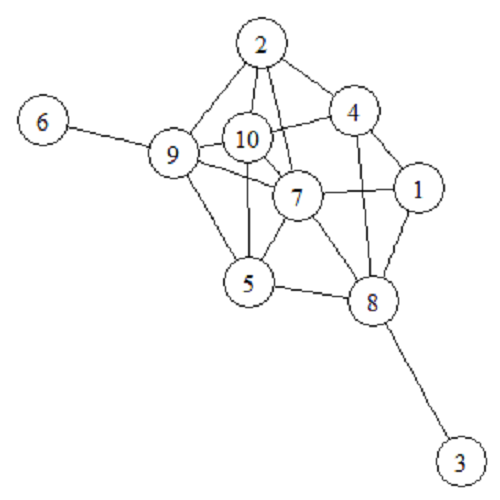
\includegraphics[width=.8\textwidth]{MaxCutGraph}
\end{minipage}
%
\begin{minipage}{.49\textwidth}
$\m{B} = \left[
\begin{array}{cccccccccc}
0 & 0 & 0 & 1 & 0 & 0 & 1 & 1 & 0 & 0\\
0 & 0 & 0 & 1 & 0 & 0 & 1 & 0 & 1 & 1\\ 
0 & 0 & 0 & 0 & 0 & 0 & 0 & 1 & 0 & 0\\
1 & 1 & 0 & 0 & 0 & 0 & 0 & 1 & 0 & 1\\
0 & 0 & 0 & 0 & 0 & 0 & 1 & 1 & 1 & 1\\
0 & 0 & 0 & 0 & 0 & 0 & 0 & 0 & 1 & 0\\
1 & 1 & 0 & 0 & 1 & 0 & 0 & 1 & 1 & 1\\
1 & 0 & 1 & 1 & 1 & 0 & 1 & 0 & 0 & 0\\
0 & 1 & 0 & 0 & 1 & 1 & 1 & 0 & 0 & 1\\
0 & 1 & 0 & 1 & 1 & 0 & 1 & 0 & 1 & 0\\
\end{array} \right]$
\end{minipage}
\caption{\emph{A graph object and associated adjacency matrix for which we would like to find the maximum cut.}}
\label{fig:maxcut}
\end{figure}

The matrix \verb!At! is constructed using the upper triangular portion of the $\m{A}_{k}$ matrices. To do this in \verb!R!, the function \verb!svec! is made available in \verb!sdpt3r!.

\begin{verbatim}
R> #Construct Ak matrices
R> A <- matrix(list(),nrow=1,ncol=n)
R> for(k in 1:n){
R>   A[[k]] <- matrix(0,nrow=n,ncol=n)
R>   diag(A[[k]])[k] <- 1
R> }

R> #Combine to form At
R> At[[1,1]] <- svec(blk[1,],A)
\end{verbatim}

Having each of the diagonal elements of $\m{X}$ constrained to be 1, \verb!b! is a $n \times 1$ matrix of ones

\begin{verbatim}
R> b <- matrix(1,nrow=n,ncol=1)
\end{verbatim}

With all the input variables now defined, we can now call \verb!sqlp! to solve the Max-Cut problem

\begin{verbatim}
R> sqlp(blk, At, C, b)
\end{verbatim}

The built-in function \verb!maxcut! takes as input a (weighted) adjacency matrix \verb!B! and returns all of the input variables required for use in \verb!sqlp!. If we wish to find to the maximum cut of the graph in Figure \ref{fig:maxcut}, given the adjacency matrix $\m{B}$ we can compute the input variables for \verb!sqlp! using \verb!maxcut!

\begin{verbatim}
R> out <- maxcut(B)
R> blk <- out$blk
R> At <- out$At
R> C <- out$C
R> b <- out$b

R> out <- sqlp(blk,At,C,b)

R> out$pobj

[1] -14.67622

R> out$X

      [,1]   [,2]   [,3]   [,4]   [,5]   [,6]   [,7]   [,8]   [,9]  [,10]
V1   1.000  0.987 -0.136 -0.858  0.480  0.857 -0.879  0.136 -0.857  0.597
V2   0.987  1.000  0.026 -0.763  0.616  0.929 -0.791 -0.026 -0.929  0.459
V3  -0.136  0.026  1.000  0.626  0.804  0.394  0.592 -1.000 -0.394 -0.876
V4  -0.858 -0.763  0.626  1.000  0.039 -0.469  0.999 -0.626  0.470 -0.925
V5   0.480  0.616  0.804  0.039  1.000  0.864 -0.004 -0.804 -0.864 -0.417
V6   0.857  0.929  0.394 -0.469  0.864  1.000 -0.508 -0.394 -1.000  0.098
V7  -0.879 -0.791  0.592  0.999 -0.004 -0.508  1.000 -0.592  0.508 -0.907
V8   0.136 -0.026 -1.000 -0.626 -0.804 -0.394 -0.592  1.000  0.394  0.876
V9  -0.857 -0.929 -0.394  0.470 -0.864 -1.000  0.508  0.394  1.000 -0.098
V10  0.597  0.459 -0.876 -0.925 -0.417  0.098 -0.907  0.876 -0.098  1.000
\end{verbatim}

Note that the value of the primary objective function is negative as we have defined $\m{C} = -(diag(\m{B}\ve{1}) - \m{B})/4$ since we require the primal formulation to be a minimization problem. The original formulation given in \cite{goemans1995improved} frames the Max-Cut problem as a maximization problem with $\m{C} = (diag(\m{B}\ve{1}) - \m{B})/4$. Therefore, the approximate value of the maximum cut for the graph in Figure \ref{fig:maxcut} is 14.68 (recall we are solving a relaxation). 

As an interesting aside, we can show that the matrix $\m{X}$ is actually a correlation matrix by considering its eigenvalues - we can see it clearly is symmetric, with unit diagonal and all elements in [-1,1].

\begin{verbatim}
R> eigen(X)$values

[1] 5.59e+00 4.41e+00 2.07e-07 1.08e-07 4.92e-08 3.62e-08 3.22e-08
[8] 1.90e-08 1.66e-08 9.38e-09
\end{verbatim}

The fact that $\m{X}$ is indeed a correlation matrix comes as no surprise. \cite{goemans1995improved} show that the set of feasible solutions for the Max-Cut problem is in fact the set of correlation matrices. So while we may not be interested in $\m{X}$ as an output for solving the Max-Cut problem, it is nonetheless interesting to see that it is in fact in the set of feasible solutions.

\bibliographystyle{plain}
\bibliography{sdpt3r}
\end{document}
